% =============================================================================
% COPYRIGHT AND DISCLAIMER
% =============================================================================
% This file is provided as a convenience template for competition participants.
% By using it, you accept full responsibility for compliance with all applicable
% copyright, licensing, and usage rules of the Association for Computing
% Machinery (ACM) and of any LaTeX packages you load (including, without
% limitation, the "acmart" document class and related ACM materials).
%
% Consult ACM's official publication, template, and copyright policies before
% using this setup for any purpose other than this competition. Do not assume
% that this template may be reused, redistributed, or submitted elsewhere
% without independently verifying ACM's current rules.
%
% Use of the "acmart" class, the "sigconf" option, or ACM-style formatting in
% this template does NOT mean that this report, this competition, its organizers,
% or any resulting PDF is sponsored, endorsed, affiliated with, or published by
% ACM. ACM trademarks and branding remain the property of ACM.
%
% Template packages live in preamble.tex.
% Citations live in main.bib. Edit this file with your paper content.
% =============================================================================

\documentclass[sigconf]{acmart}
% =============================================================================
% Template setup — participants normally do not edit this file.
% Author content belongs in main.tex; citations belong in main.bib.
% \documentclass lives in main.tex so Overleaf does not treat this file as root.
% =============================================================================

% --- Competition / non-ACM-submission friendly rights metadata -------------
\setcopyright{none}
\settopmatter{printacmref=false}
\acmConference[Kaggle Competition]{Filament Segmentation Challenge}{2026}{\href{https://www.kaggle.com/competitions/filament-segmentation-2026}{kaggle.com/competitions/filament-segmentation-2026}}
\acmBooktitle{Competition Report}
\acmDOI{}
\acmISBN{}

% --- Author guidance text --------------------------------------------------
% \guide{...} is gray italic while \guideStyletrue; omitted from the PDF if false.
% Flip the switch in main.tex after % =============================================================================
% Template setup — participants normally do not edit this file.
% Author content belongs in main.tex; citations belong in main.bib.
% \documentclass lives in main.tex so Overleaf does not treat this file as root.
% =============================================================================

% --- Competition / non-ACM-submission friendly rights metadata -------------
\setcopyright{none}
\settopmatter{printacmref=false}
\acmConference[Kaggle Competition]{Filament Segmentation Challenge}{2026}{\href{https://www.kaggle.com/competitions/filament-segmentation-2026}{kaggle.com/competitions/filament-segmentation-2026}}
\acmBooktitle{Competition Report}
\acmDOI{}
\acmISBN{}

% --- Author guidance text --------------------------------------------------
% \guide{...} is gray italic while \guideStyletrue; omitted from the PDF if false.
% Flip the switch in main.tex after % =============================================================================
% Template setup — participants normally do not edit this file.
% Author content belongs in main.tex; citations belong in main.bib.
% \documentclass lives in main.tex so Overleaf does not treat this file as root.
% =============================================================================

% --- Competition / non-ACM-submission friendly rights metadata -------------
\setcopyright{none}
\settopmatter{printacmref=false}
\acmConference[Kaggle Competition]{Filament Segmentation Challenge}{2026}{\href{https://www.kaggle.com/competitions/filament-segmentation-2026}{kaggle.com/competitions/filament-segmentation-2026}}
\acmBooktitle{Competition Report}
\acmDOI{}
\acmISBN{}

% --- Author guidance text --------------------------------------------------
% \guide{...} is gray italic while \guideStyletrue; omitted from the PDF if false.
% Flip the switch in main.tex after \input{preamble}.
%
% Do not use \guide{...} for \email{...}.
\usepackage{xcolor}
\newif\ifguideStyle
\guideStyletrue
\newcommand{\guide}[1]{%
  \ifguideStyle
    {\color{gray!65}\itshape #1}%
  \fi
}

% --- Math ------------------------------------------------------------------
% Do NOT load amssymb (or amsfonts): acmart already loads newtxmath, which
% defines the same symbols (e.g. \Bbbk) and causes a conflict on Overleaf.
% amsmath is already provided by acmart; mathtools extends it.
\usepackage{mathtools}

% --- Figures ---------------------------------------------------------------
% graphicx is already loaded by acmart
\usepackage{subcaption}

% --- Tables ----------------------------------------------------------------
% booktabs is already loaded by acmart
\usepackage{tabularx}
\usepackage{multirow}

% --- Bibliography style is set in main.tex (ACM-Reference-Format) ----------
.
%
% Do not use \guide{...} for \email{...}.
\usepackage{xcolor}
\newif\ifguideStyle
\guideStyletrue
\newcommand{\guide}[1]{%
  \ifguideStyle
    {\color{gray!65}\itshape #1}%
  \fi
}

% --- Math ------------------------------------------------------------------
% Do NOT load amssymb (or amsfonts): acmart already loads newtxmath, which
% defines the same symbols (e.g. \Bbbk) and causes a conflict on Overleaf.
% amsmath is already provided by acmart; mathtools extends it.
\usepackage{mathtools}

% --- Figures ---------------------------------------------------------------
% graphicx is already loaded by acmart
\usepackage{subcaption}

% --- Tables ----------------------------------------------------------------
% booktabs is already loaded by acmart
\usepackage{tabularx}
\usepackage{multirow}

% --- Bibliography style is set in main.tex (ACM-Reference-Format) ----------
.
%
% Do not use \guide{...} for \email{...}.
\usepackage{xcolor}
\newif\ifguideStyle
\guideStyletrue
\newcommand{\guide}[1]{%
  \ifguideStyle
    {\color{gray!65}\itshape #1}%
  \fi
}

% --- Math ------------------------------------------------------------------
% Do NOT load amssymb (or amsfonts): acmart already loads newtxmath, which
% defines the same symbols (e.g. \Bbbk) and causes a conflict on Overleaf.
% amsmath is already provided by acmart; mathtools extends it.
\usepackage{mathtools}

% --- Figures ---------------------------------------------------------------
% graphicx is already loaded by acmart
\usepackage{subcaption}

% --- Tables ----------------------------------------------------------------
% booktabs is already loaded by acmart
\usepackage{tabularx}
\usepackage{multirow}

% --- Bibliography style is set in main.tex (ACM-Reference-Format) ----------


% Guide styling: \guideStylefalse = show gray italic hints; \guideStylefalse = omit them
\guideStylefalse
% \guideStylefalse


\setlength{\emergencystretch}{1em}

\begin{document}
\title{A Reproducible U-Net Baseline with Grouped Validation}
\subtitle{A Solution to the Solar Filament Segmentation Challenge 2026}
\author{Srivatsav Kannan}

\begin{abstract}
This report describes our solution to the Solar Filament Segmentation Challenge~2026, a Kaggle competition on automatic segmentation of solar filaments in GONG H-$\alpha$ observations.
We train a compact, single-channel U-Net from scratch using only competition-approved labels. Independent annotator unions form soft foreground targets; annotators remain separate in the official instance-aware evaluation. Physical observations are grouped into temporal folds with an embargo. Calibration determines the model and native-resolution instance reconstruction before a protected holdout is opened. The frozen baseline achieves holdout Panoptic Quality (PQ) of 0.3462 (physical-image bootstrap 95\% interval: 0.3288--0.3633). We provide modular code, exact package versions, a canonical notebook, checkpoint hashes, visual diagnostics, and fail-closed submission checks. This is a development baseline, not a claim of a final winning method.
\end{abstract}
\maketitle
\section{Introduction}
    This report goes over the details of our submitted solution to the Solar Filament Segmentation Challenge~2026 \cite{filament-segmentation-2026}. The challenge, launched on July~10,~2026, is organized by the Earth-Space AI Research (ESAIR) Lab\footnote{\href{https://www.esairlab.com/home}{www.esairlab.com/}}. This challenge utilizes the MAGFiLO dataset for evaluation of the segmentation algorithms \cite{ahmadzadeh2024dataset}.
Our contribution is a reproducible experimental foundation that makes data provenance, annotator dependence, instance errors, and evaluation uncertainty explicit. A semantic mask alone does not solve the task: gaps can fragment one filament, while bridges can merge distinct filaments. We therefore measure the complete foreground-to-instance pipeline with the organizer's released evaluator rather than select by pixel Dice alone. All experiments in this report were conducted on 6 September 2026. The separate final-entry form and final candidate selection remain pending.

\section{Methodology}\label{sec:methodology}
\subsection{Inputs, annotation policy, and splits}
The supplied bundle contains 707 physical training JPEGs and 180 test JPEGs, all $2048\times2048$ grayscale pixels. There are 1,154 annotator-image records and 8,199 instance polygons. Each file can have several independent annotators; splitting these records separately would leak the same observation across partitions. The four chirality categories do not change the single-class output contract.

We use only \path{MAGFiLO_1.0_Annotations_kaggle2026_train.json}. The full public MAGFiLO annotation release overlaps competition test observations and is excluded. No external training images, pretrained weights, manually corrected test masks, filename-based predictions, or auxiliary inference metadata are used. The annotation file and every input file are SHA-256 hashed. Decoded pixels are additionally hashed to find exact duplicates; none were found across train and test.

We assign physical observations to five deterministic grouped folds (seed 2026), using 27-day blocks anchored at 1 January 2010. Blocks connected by exact pixel duplicates would be united. Fold 0 is holdout, fold 1 calibration, and the other folds are optimization data after removing observations within three days of either evaluation partition. The resulting counts are 399 training, 149 calibration, 145 holdout, and 14 embargoed images. This protocol reduces short-range leakage; it does not prove independence of structures persisting beyond the embargo or recurring across rotations. The held-out images span the six GONG site suffixes present in the bundle.

\subsection{Targets and preprocessing}
For each annotator, polygon masks are rasterized with the COCO API and combined into a binary foreground union. These independent unions are averaged, giving a per-pixel soft target that retains disagreement instead of treating annotators as separate training samples. BOX downsampling preserves partial coverage; targets are cached as 8-bit probabilities. Evaluation never averages or unions annotator ground truths.

JPEG intensities are converted to one luminance channel, scaled to $[0,1]$, resized bilinearly to $1024\times1024$, then normalized by $(x-0.5)/0.25$. We do not apply additional limb flattening: the dataset's JPEG generation already modifies large-scale intensity variation. Half the crops are sampled around a foreground location and half uniformly; physical images are sampled uniformly. Rotations by multiples of 90 degrees, flips, modest gain/offset perturbations, and occasional weak Gaussian blur provide augmentation. No test-time visual edits are made.

\subsection{Model and optimization}
The baseline follows U-Net's encoder--decoder and skip-connection design~\cite{unet}. At each scale, two $3\times3$ convolutions use GroupNorm and SiLU. Three downsampling stages yield widths $w,2w,4w,8w$; bilinear upsampling and concatenated skips restore resolution. A $1\times1$ head produces one foreground logit. The selected model uses width 24 and 384-pixel crops. A second compact configuration provides a calibration comparator; all variants use the same physical-image split.

We minimize binary cross-entropy plus soft Dice loss with AdamW, learning rate $10^{-3}$, weight decay $10^{-4}$, a cosine schedule to $10^{-5}$, batch size six, and gradient clipping at one. Training stops after 6,000 updates chosen before holdout inspection. The selected run took 1227.3 seconds on local Apple Silicon with 24 GB unified memory, excluding input preparation. This time is specific to this hardware and implementation, and is not a benchmark against published models. Seeds, configuration, loss history, checkpoint checksum, and environment versions accompany the release.

\begin{figure*}[t]
\centering
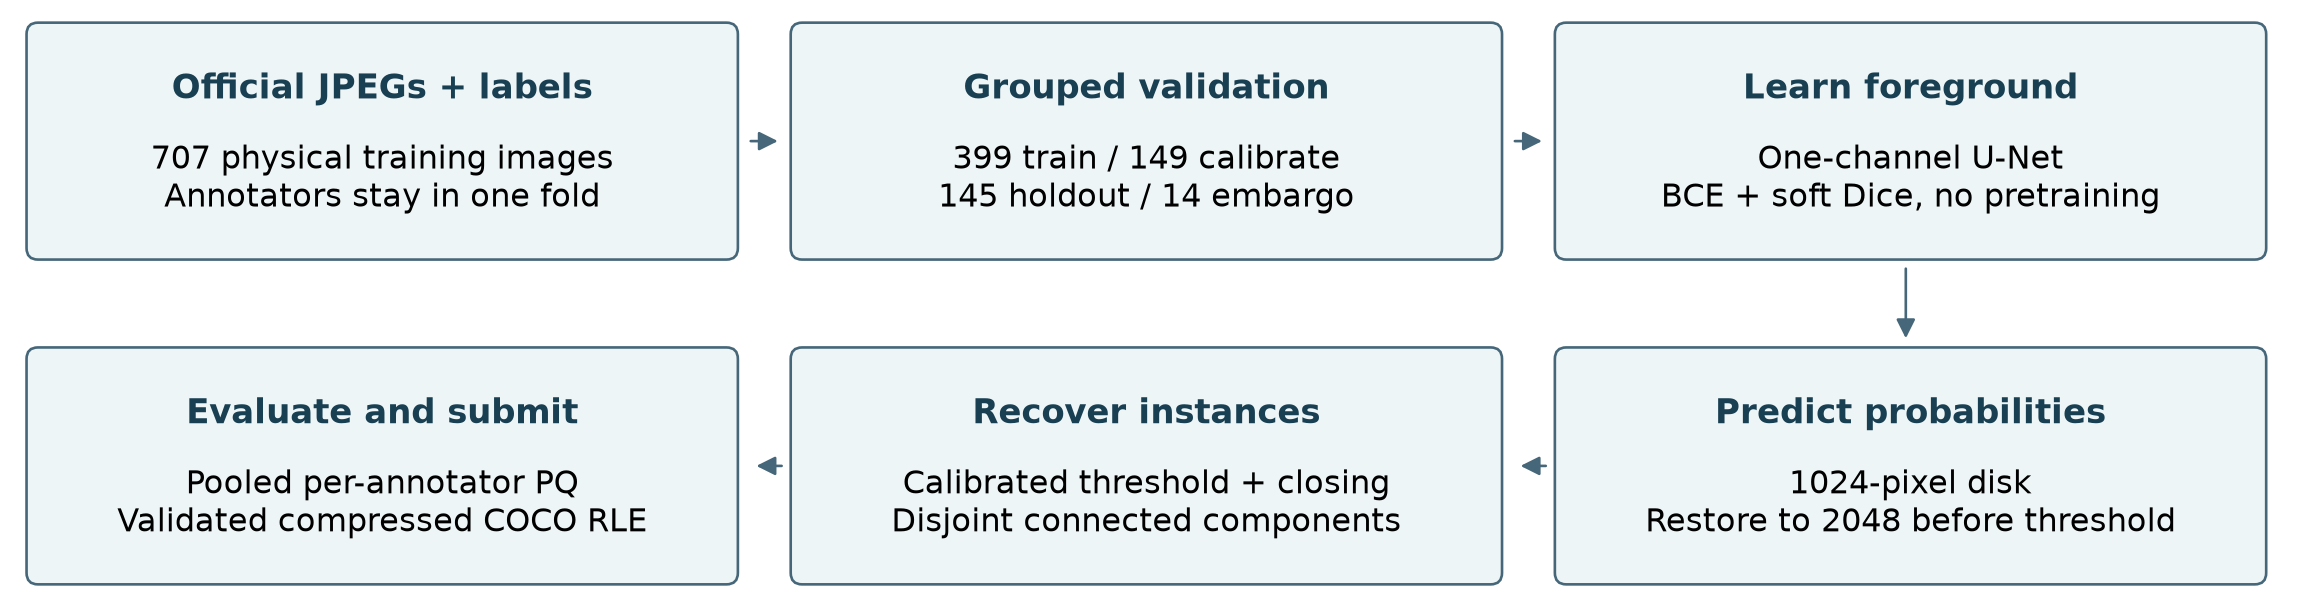
\includegraphics[width=\textwidth]{../figures/pipeline.png}
\caption{Implemented workflow. Every annotator and crop of one physical observation follows the same fold. Thresholds and instance reconstruction are chosen on calibration before holdout evaluation.}
\Description{Official data passes through grouped splitting, U-Net foreground learning, probability inference, disjoint instance reconstruction, and evaluated COCO output.}
\end{figure*}

\subsection{Inference and instance reconstruction}
The selected checkpoint is evaluated on the complete resized disk. Four flip predictions are averaged.
Probabilities are bilinearly restored to $2048\times2048$ before thresholding. Calibration selected threshold 0.6, a disk-shaped binary closing radius of 3 native pixels, and minimum component area 400 native pixels. Eight-connected foreground components become instances. This guarantees exclusive pixel ownership but cannot separate touching filaments without an additional instance representation. The area cutoff suppresses spurious fragments at the cost of small-object recall.

Each nonempty component is encoded as compressed COCO RLE using a Fortran-contiguous byte array. Output has precisely two columns, \texttt{filament\_id} and \texttt{segmentation\_rle}, with one row per instance and the original filename stem preserved. A sidecar records coverage of all 180 images, including zero detections. Preflight rejects invalid probabilities, empty masks, duplicates, overlaps, unknown IDs, and incomplete coverage.

\section{Evaluation}\label{sec:evaluation}
\subsection{Metric fidelity and candidate selection}
We reproduce the released organizer implementation of PQ~\cite{panoptic}. For each physical image, one prediction set is compared with each annotator separately. Pairs with strictly greater than 0.5 IoU qualify; matched IoUs, TP, FP, and FN are pooled across annotator-image entries:
\[
\mathrm{PQ}=\frac{\sum_{\mathrm{matched}}\mathrm{IoU}}{\mathrm{TP}+0.5\mathrm{FP}+0.5\mathrm{FN}}.
\]
We retain the official all-qualifying-pairs behavior where GT overlaps complicate textbook one-to-one assumptions. Background is excluded. Numerical parity tests compare the efficient COCO-RLE implementation with the organizer's tensor functions, including empty sets and the strict threshold. Additional tests cover polygon conversion, asymmetric RLE round trips, split/merge penalties, temporal grouping, inference tiling, and CSV ownership.

The initial postprocessing grid contained 16 settings. After excess calibration false positives were observed, nine settings with larger area cutoffs were added. The compact full-frame model improved from PQ 0.25096 to 0.27503 under this adaptive search; the classical local-background-deficit reference reached 0.08265. Expanded capacity/context and overlapping-tile inference were then compared on calibration. The selected candidate reached 0.3314. These maxima are optimistically biased by tuning; they are not independent validation estimates. The model, inference mode, thresholds, and split checksum were frozen before opening holdout results.

\begin{table}[t]
\centering
\caption{Frozen candidate on 145 protected physical images. Counts pool independent annotator comparisons. The interval resamples physical images 1,000 times.}
\begin{tabular}{lr}
\toprule
Measure & Value \\
\midrule
PQ & 0.3462 \\
95\% bootstrap interval & [0.3288, 0.3633] \\
Segmentation quality (SQ) & 0.6603 \\
Recognition quality (RQ) & 0.5244 \\
TP / FP / FN & 952 / 1065 / 662 \\
Fragmented GT / merged predictions & 144 / 29 \\
\bottomrule
\end{tabular}
\end{table}

\subsection{Uncertainty and failure analysis}
All annotator comparisons of one physical observation are retained together during bootstrap resampling. This reflects physical-image sampling variability, but does not capture every temporal dependence, random-seed effect, or adaptive research decision. Site-specific intervals and overlap distributions are included in the repository. Positive-pair IoU/Dice plots exclude zero pairs explicitly; misses remain visible in FP/FN counts. Size-stratified recall uses native-area bins below 1,000, 1,000--10,000, and at least 10,000 pixels.

\begin{figure*}[t]
\centering
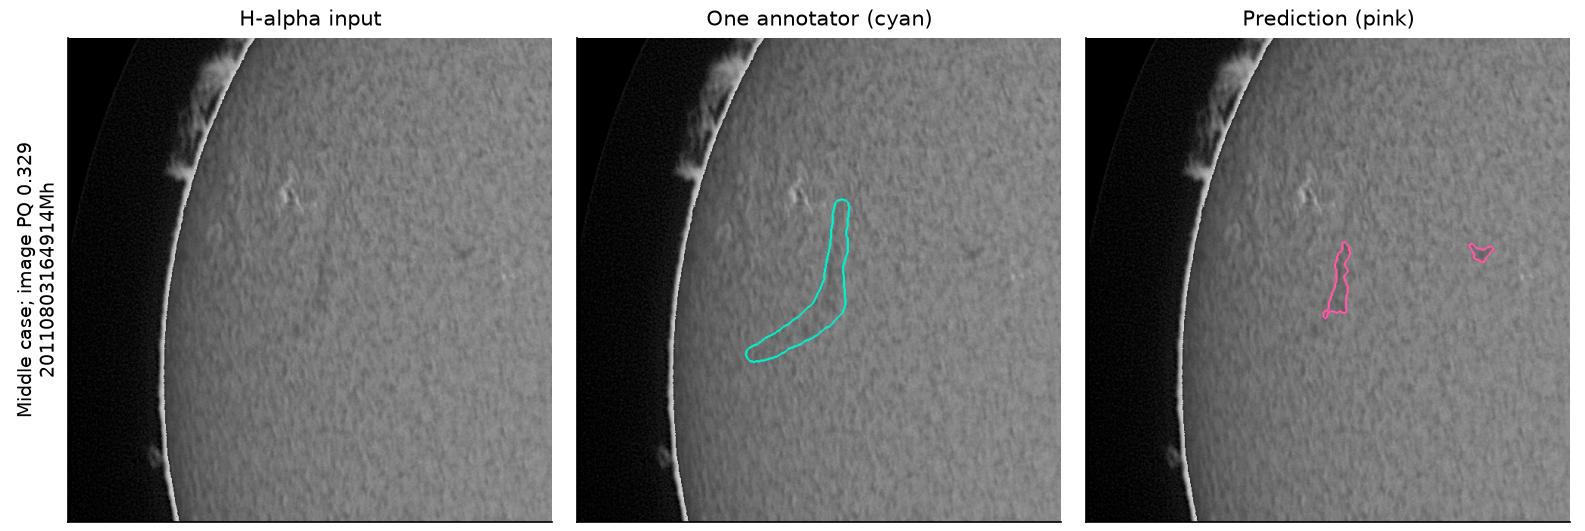
\includegraphics[width=\textwidth]{../figures/report-example.png}
\caption{Systematically selected median calibration case, cropped around the largest instance of the first supplied annotator. Cyan shows that annotator; pink shows predictions. The full repository gallery also includes worst and best cases selected by physical-image PQ.}
\Description{A grayscale H-alpha crop alongside annotator boundaries and predicted filament boundaries.}
\end{figure*}

\begin{figure*}[t]
\centering
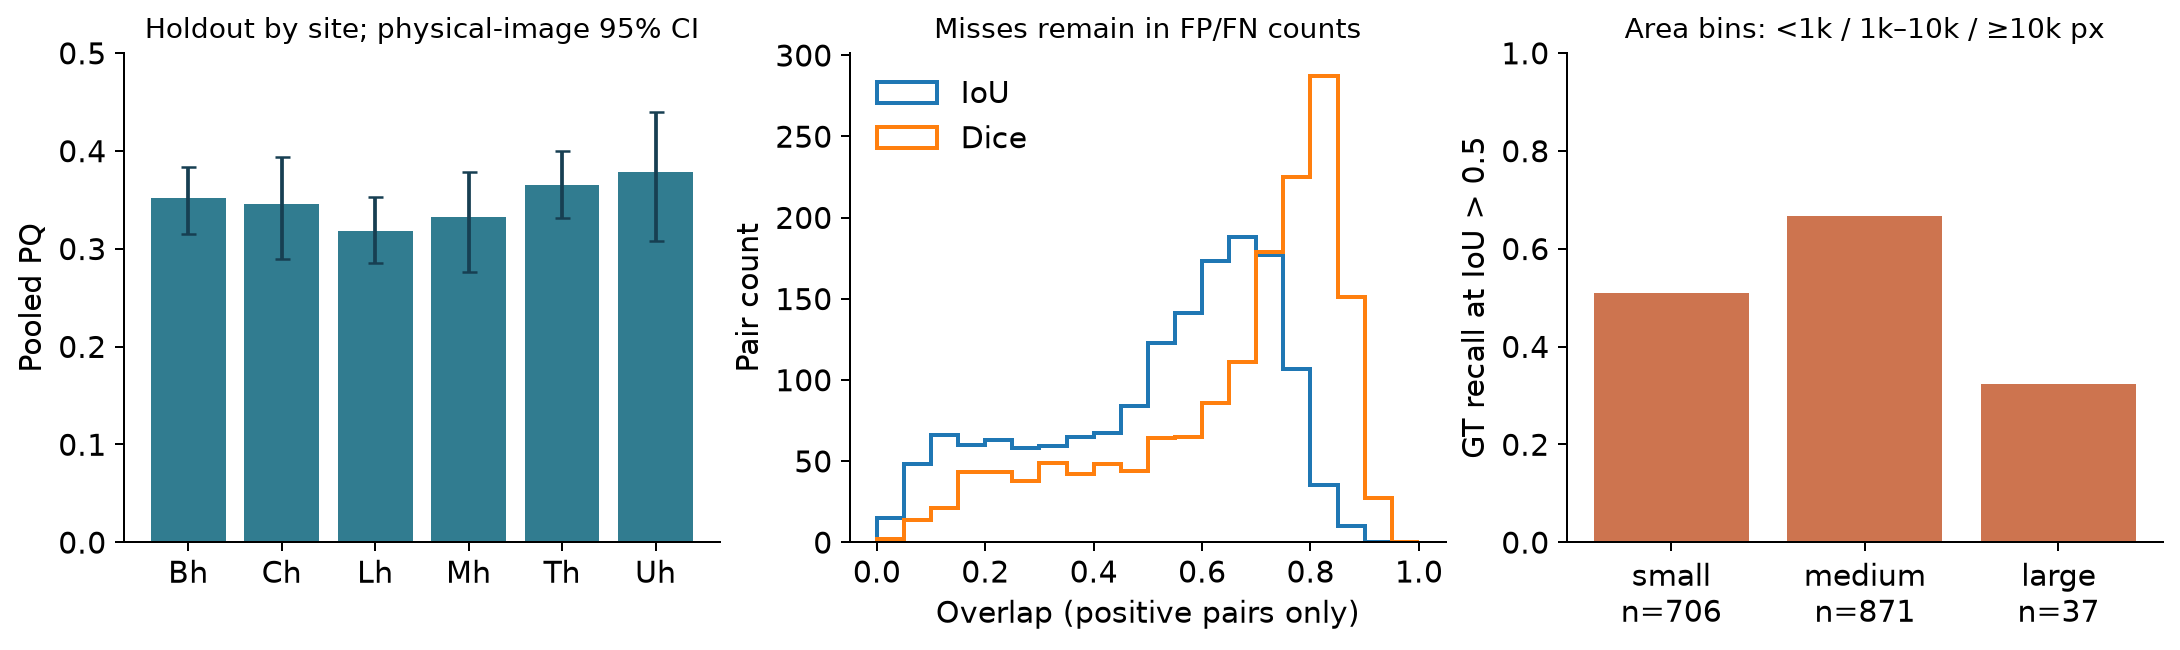
\includegraphics[width=\textwidth]{../figures/holdout-diagnostics.png}
\caption{Protected holdout diagnostics. Left: site-wise pooled PQ and physical-image bootstrap intervals. Middle: positive-pair overlap distributions; missing objects remain in FP/FN counts. Right: GT recall by native mask area, showing size-dependent misses.}
\Description{Six site-specific PQ estimates with confidence intervals, IoU and Dice distributions, and recall in three instance-size bins.}
\end{figure*}

Our principal limitations are missing faint structures, false positives on other dark features, boundary mismatch, and imperfect connected-component identity. Only 12 of 37 large annotated masks are matched, supporting targeted work on truncation and fragmentation. Independent annotators also disagree about extent and completeness. We preserve the official metric despite its penalties for some physically plausible but unannotated detections. Visual review therefore accompanies quantitative validation. A high pixel overlap is insufficient if the output breaks one object into many fragments or joins distinct objects.

Edge-guided attention~\cite{edgeattnet}, explicit mask-set prediction~\cite{mask2former}, and skeleton-aware losses~\cite{cldice} motivate subsequent controlled experiments. None is implemented in this baseline. Our next priority is native-resolution detail and boundary/affinity supervision, followed by a detector-plus-refiner comparison. Stricter chronological and site-held-out tests, near-duplicate auditing, additional training seeds, and a paired uncertainty analysis are needed before stronger generalization claims. Published Dice or pairwise mIoU values are not compared directly with this competition's PQ.

\subsection{Reproduction and release status}
The public source repository is \url{https://github.com/srivatsav-kannan/solar-seg}. Its canonical notebook imports the same modules used by the CLI and contains the audit, target construction, training, calibration, evaluation, inference, and serialization workflow. Release inference uses a pinned source revision and a checksummed checkpoint. CPU replay records environment and output hashes; exact bitwise equality across processor architectures is not assumed. Submission gates bind correctness checks, candidate selection, holdout results, morphology review, and notebook replay to the exact CSV.

The source is MIT licensed; competition data and host template material retain their original terms. Raw images, annotations, credentials, and undocumented external weights are excluded from Git history. This development report describes the measured baseline only. Final contact metadata, the competition's Google form, and final submission selection must be completed before the deadline; the repository must remain accessible through the winner announcement.


\clearpage
\section{Acknowledgment}\label{sec:acknowledgment}
    % Do not change
    The organization of the Filament Segmentation Challenge 2026 is partially supported by the U.S. National Science Foundation (NSF) under Grant No. 2209912 and 2433781, directorate for Computer and Information Science and Engineering (CSE), and Office of Advanced Cyberinfrastructure (OAC), and Grant No. 2511630, AST Division Of Astronomical Sciences and MPS Directorate for Mathematical and Physical Sciences.

    The Filament Segmentation Challenge 2026 is sponsored by the U.S. National Science Foundation (NSF) National Solar Observatory (NSO).

    This work utilizes GONG data obtained by the NSO Integrated Synoptic Program, managed by the National Solar Observatory, which is operated by the Association of Universities for Research in Astronomy (AURA), Inc. under a cooperative agreement with the National Science Foundation and with contribution from the National Oceanic and Atmospheric Administration. The GONG network of instruments is hosted by the Big Bear Solar Observatory, High Altitude Observatory, Learmonth Solar Observatory, Udaipur Solar Observatory, Instituto de Astrofísica de Canarias, and Cerro Tololo Interamerican Observatory.

\bibliographystyle{ACM-Reference-Format}
\bibliography{main}

\end{document}
